\documentclass{article}

\usepackage{graphicx}
\usepackage{array}
\usepackage{amsfonts}
\usepackage{amsmath}
\usepackage{geometry}
\usepackage{float}


\geometry{hmargin=2.5cm,vmargin=1.5cm}

\title{INDENG 242 : Homework 1}
\author{Arnaud Minondo}

\begin{document}
    \maketitle
    \section*{Problem 1}
    Let $\hat{\beta} = \frac{\sum_{j=1}^n x_jy_j}{\sum_{j=1}^nx_j^2}$ and $ \hat{y_i} = x_i\hat{\beta}$ so :
    \\\\
    $\hat{y_i} = x_i\frac{\sum_{j=1}^n x_jy_j}{\sum_{k=1}^nx_k^2} = x_i \sum_{j=1}^n\frac{x_j}{\sum_{k=1}^nx_k^2}y_j = \sum_{j=1}^n\frac{x_ix_j}{\sum_{k=1}^nx_k^2}y_j =\sum_{j=1}^na_jy_j $
    where $a_j = \frac{x_jx_i}{\sum_{k=1}^nx_k^2}$.
    \\
    \section*{Problem 2}
    \subsection*{2.$i$}
    Let $p(X) = \frac{\exp(\beta_0+\beta_1X)}{1+\exp(\beta_0+\beta_1X)}$ we want to show that $\frac{p(X)}{1-p(X)} = \exp(\beta_0+\beta_1X)$
    \\\\
    ${ \frac{p(X)}{1-p(X)} = \frac{\frac{\exp(\beta_0+\beta_1X)}{1+\exp(\beta_0+\beta_1X)}}{1-\frac{\exp(\beta_0+\beta_1X)}{1+\exp(\beta_0+\beta_1X)}} = \frac{\frac{\exp(\beta_0+\beta_1X)}{1+\exp(\beta_0+\beta_1X)}}{\frac{1+\exp(\beta_0+\beta_1X)-\exp(\beta_0+\beta_1X)}{1+\exp(\beta_0+\beta_1X)}}=\exp(\beta_0+\beta_1X)}$.
    \\\\
    Now suppose $\frac{p(X)}{1-p(X)} = e^{\beta_0+\beta_1X}$ then : $ p(X) = (1-p(X))e^{\beta_0+\beta_1X}$ so $p(X)(1+e^{\beta_0+\beta_1X}) = e^{\beta_0+\beta_1X}$
    \\
    Finally : $p(X) = \frac{e^{\beta_0+\beta_1X}}{1+e^{\beta_0+\beta_1X}}$ so the two expressions are equivalent.
    \subsection*{2.$ii$}
    Let 
    $\mathcal{L}(\beta) = \prod_{i=1}^n \mathbb{P}(Y=y_i|x_i,\beta) = \prod_{i=1}^n(p(x_i)^{y_i}(1-p(x_i))^{1-y_i})$\\
    As $\log$ is an increasing function, maximizing the likelihood or the $\log$ of the likelihood is the same.\\
    $\log(\mathcal{L}(\beta)) = \sum_{i=1}^n y_i\log(p(x_i))+(1-y_i)\log(1-p(x_i)) = \sum_{i=1}^n y_i \log(\frac{e^{\beta^Tx_i}}{1+e^{\beta^Tx_i}}) + (1-y_i)\log(\frac{1}{1+e^{\beta^Tx_i}})$\\
    $ = \sum_{i=1}^ny_i\beta^Tx_i-y_i\log(1+e^{\beta^T x_i})-(1-y_i)\log(1+e^{\beta^Tx_i}) = \sum_{i=1}^n y_i\beta^Tx_i-\log(1+e^{\beta^Tx_i})$\\
    The optimization problem is : find $\hat{\beta} = \arg\max_{\beta}(\log(\mathcal{L}(\beta))) = \arg\min_{\beta}(\sum_{i=1}^n\log(1+e^{\beta^Tx_i})-y_i\beta^Tx_i)$.
    \\
    To solve this we need to differentiate with respect to $\beta$ and obtain that $\sum_{i=1}^n \frac{x_i}{1+\exp(-\beta^Tx_i)} - y_ix_i = 0 $
    \subsection*{2.$iii$}
    We can notice that when $\beta^Tx > 0$ then $p(x)>1-p(x)$ and if  $\beta^Tx < 0$ then $p(x)<1-p(x)$.
     As we would predict the label which is the most probable following estimation $p$ then $\beta$ represents the plan
     separating best the datas into the two classes.
    \section*{Problem 3 : Framingham Heart study}
    \subsection*{3.a.$ii$}
    The parameter model $\beta$ for my model is : $\beta = 
    \left(
    \begin{array}{lr}
        \text{male } & 0.52 \\
        \text{age } & 0.03 \\
        \text{currentSmoker } & -0.16 \\
        \text{cigsPerDay } & 0.016 \\
        \text{BPMeds } & 0.11 \\
        \text{prevalentStroke } & 0.075 \\
        \text{prevalentHyp } & 1.06 \\
        \text{diabetes } & 0.20 \\
        \text{totChol } & -0.001 \\
        \text{sysBP } & 0.01 \\
        \text{diaBP } & -0.04 \\
        \text{BMI } & -0.04 \\
        \text{heartRate } & -0.02 \\
        \text{glucose } & 0.004 \\
        \text{intercept } & -0.42 \\
    \end{array}
    \right)$
    \\\\
    Let $X$ be the matrix composed of all samples with all features organized in the same order as $\beta$ describe above then
    $p(x) = \frac{1}{1+e^{-\beta^T x}}$ represents the probability that x is of class 1 ie. is going to developp a coronary heart disease in the next en years.
    \\

    \subsection*{3.a.$iii$}
    The basic logistic regression on the testing set has an accuracy of : 0.84\%. This is basically the performance of a dummy model.
    Its TPR is : 0.11 and FPR is :0.01 which are not good at all.

    \subsection*{3.b.$i$}
    
    \begin{figure}[H]
        \center
        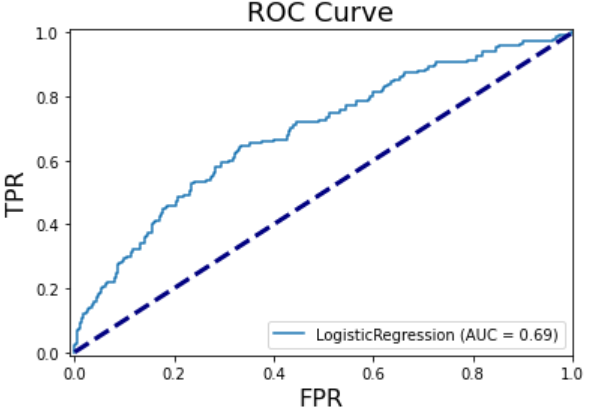
\includegraphics{ROC_curve.png}
        \caption{ROC Curve}
        \label{ROC Curve}
    \end{figure} 
    \newpage
    \subsection*{3.b.$ii$}
    \begin{figure}[H]
        \center
        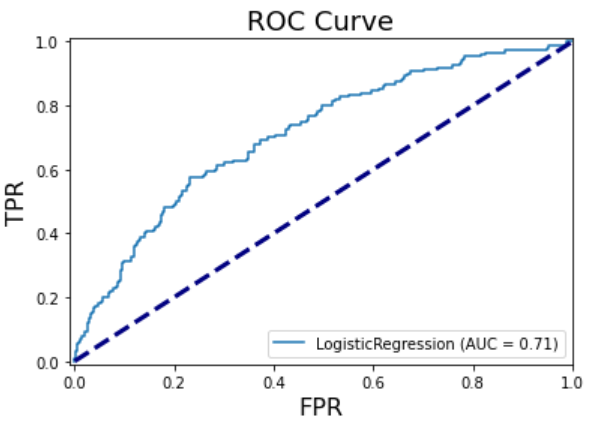
\includegraphics{ROC_curve_bal.png}
        \caption{Roc Curve Balanced model}
    \end{figure}
    \subsection*{3.b.$iii$}
    The two models behave differently. The basic model has a lot of False Positive because of the imbalance, whereas there
     are loads less false positive for the balanced model. There are more False positive

    \section*{Problem 4 : Nissan Rogue Sales Study}
    \subsection*{4.a}
    $i$.
    It is important to keep track of the time dependance because the model is going to predict with an increasing time.
    \\
    If the time data is not given with the others corresponding time datas then the time would just be a noise without meaning
    for the regression.
    \\
    In keeping the order, the subjacent logic is kept. 
    \\\\\\\\
    $ii$.
    Let X be the matrix containing all samples and Y the vector containing all regression values.\\
    Our model using all datas :\\ $\beta = (XX^T)^{-1}XY = \left(\begin{array}{lr}
        \text{MonthNumeric } & -2.546 *10^5 \\
        \text{Year } & 7657\\
        \text{Unemployment } & -1523 \\
        \text{RogueQueries } & 202 \\
        \text{CPIAll } & -1807 \\
        \text{CPIEnergy } & 126 \\
        \text{August } & 1.024*10^6 \\
        \text{December } & 2.046*10^6 \\
        \text{February } & -5.074*10^5 \\
        \text{January } & -7.65*10^5 \\
        \text{July } & 7.667*10^5 \\
        \text{June } & 5.13*10^5 \\
        \text{March } & -2.499*10^5 \\
        \text{May } & 2.588*10^5 \\
        \text{November } & 1.787*10^6 \\
        \text{October } & 1.532*10^6\\
        \text{September } & 1.279*10^6\\
        \text{Intercept } & -1.399*10^7\\
    \end{array}\right)$ with intercept : $-1.399*10^7$.\\\\
    A prediction would be  : $y =\text{intercept} + \beta^Tx$ where $x$ is a vector containing all informations (MonthNumeric, Year, Unemployement,...) to estimate the sales.
    \\\\
    $iii$.
    The model has $OSR^2 = 1- \frac{RSS}{TSS} = 0.82$.\\
     $TSS = \frac{1}{m}\sum\limits_{i=1}^m (y_i-\overline{y})^2$ which is the variance of the testing regression values sequence. 
     $RSS =  \frac{1}{m}\sum\limits_{i=1}^m(\hat{y_i}-y_i)^2$ which is the sum of the errors squared. The $RSS = TSS$ iff the model predicts the mean. $R^2$ measures the efficiency of our model in comparison with a dummy model which would always predict the mean.
    \subsection*{4.b}
    $i$. The VIF test reveals that MonthNumeric and each Mounth column (
     January, February, March, ...) are perfectly coralated because :
     MonthNumeric = January + 2February + 3 March+...+ 12 December.
     That's why I dropped MonthNumeric. It also reveals that year and RogueQueries are related with other variables. 
     So I first dropped Year and all values seem to have a reasonable VIF.
    \\\\
    It is important because the coefficient of a feature that has a high VIF introduces high variance as it depends of other features. Ex : $y = 2x_1 + 3x_2 = 3x_1 + 2x_2 = 5x_2$ if $x_1=x_2$.
    \\\\
    $ii$.
    Using the p-values to estimate whether a coefficient is good or not I dropped all months except December and March. 

    I tried dropping the intercept. I thought that RogueQueries have a big correlation with rogue sales and indeed in the training set,
    training only with respect to RogueQueries gives good approximations. A R-Squared of 0.95 but it is charactheristic of overfitting because 
    the OSR is 0.76 which is a bit less than the older model.
    
    Using the covariance matrix of the database I concluded that CPIEnergy, MonthNumeric and Unemployement were highly correlated which is not very intuitive.
    That's why my final model only involves one of the three.
    \\\\
    $iii$.
    The model performs a lot better on the training set with an R-squared of 0.95, we have to be carefull about overfitting.
    It turns out that the OSR is 0.72 which is worse than the original model but adjusting both OSR
    and we have better adjusted OSR-squared of 0.65 for our new model and 0.60 for the older one. It could be beneficial
    to only use RogueQueries without intercept.

    We notice that a feature with a negative weight will reduce the number of sale of a given sample. This is the case for :
    Unemployment, CPIEnergy.
    At contrary, a feature with a positive weight will increase the number of sale of a given sample. this is the case for :
    RogueQueries, CPIAll, December, March, August.
    Other features don't have a clear impact on the sales, either very low correlation with RogueSales, either an impact through another variable.

    \end{document}